\pagestyle{empty}
\chapter*{\centering \large DAFTAR RIWAYAT HIDUP}
\thispagestyle{empty}

\begin{wrapfigure}{l}{4cm}
	\vspace{-25pt}
	\begin{center}
		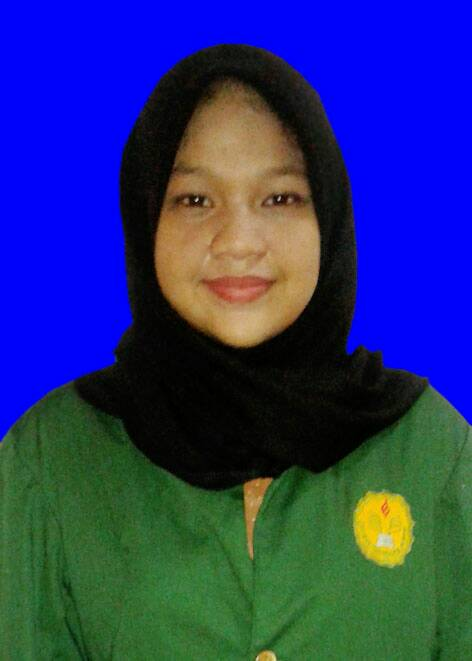
\includegraphics[width=0.27\textwidth]{gambar/pas-foto}
	\end{center}
	\vspace{-80pt}
\end{wrapfigure}

\noindent \textbf{SAULIA KARINA.}  Lahir di Jakarta, 27 Juni 1997  Anak pertama dari pasangan Bapak Syarifudin dan Ibu Ana Yohana. Saat ini beralamatkan di Jl. Pisangan Baru I RT.006 RW.08 No.4, Kecamatan Matraman Jakarta Timur.

\vspace{0.5cm}
\noindent
\begin{center}
	\begin{flushright}
		\begin{tabular}{lcl}
			No. Ponsel	& :&  083843549167 \\
			Email	& :&  sauliakarina@gmail.com
		\end{tabular}
	\end{flushright}
\end{center}
\vspace{0.5cm}

\noindent \textbf{Riwayat Pendidikan} : Penulis mengawali pendidikan di TK Nurul Iman pada tahun 2002 - 2003, dan kemudian melanjutkan pendidikan di SDN Pisangan Baru 01 Pagi pada tahun 2003 - 2009. Setelah itu, penulis melanjutkan ke SMPN 7 Jakarta hingga tahun 2012. Kemudian melanjutkan ke SMAN 54 Jakarta pada tahun 2012-2015. Di Tahun 2015 penulis melanjutkan ke Universitas Negeri Jakarta (UNJ), Program Studi Ilmu Komputer, melalui jalur PENMABA. Di akhir tahun 2019 (Kamis, 09 Agustus 2018) penulis telah memperoleh gelar Sarjana Komputer (S.Kom), Program Studi Ilmu Komputer, Fakultas Matematika dan Ilmu Pengetahuan Alam, Universitas Negeri Jakarta.

\noindent \textbf{Riwayat Organisasi} : Selama di bangku perkuliahan, penulis aktif di Badan Eksekutif Mahasiswa Rumpun Matematika sebagai staff di Departemen Advokasi dan Keolahragaan kemudian melanjutkan di BEM FMIPA dengan departemen yang sama. Penulis juga berpartisipasi dalam kegiatan BINER (Be Innovative and Educated Researcher) yaitu kegiatan workshop dan seminar yang diadakan oleh DEFAULT, dimana penulis tergabung sebagai anggota merangkap Bendahara. 